% Options for packages loaded elsewhere
\PassOptionsToPackage{unicode}{hyperref}
\PassOptionsToPackage{hyphens}{url}
%
\documentclass[
]{article}
\usepackage{lmodern}
\usepackage{amssymb,amsmath}
\usepackage{ifxetex,ifluatex}
\ifnum 0\ifxetex 1\fi\ifluatex 1\fi=0 % if pdftex
  \usepackage[T1]{fontenc}
  \usepackage[utf8]{inputenc}
  \usepackage{textcomp} % provide euro and other symbols
\else % if luatex or xetex
  \usepackage{unicode-math}
  \defaultfontfeatures{Scale=MatchLowercase}
  \defaultfontfeatures[\rmfamily]{Ligatures=TeX,Scale=1}
\fi
% Use upquote if available, for straight quotes in verbatim environments
\IfFileExists{upquote.sty}{\usepackage{upquote}}{}
\IfFileExists{microtype.sty}{% use microtype if available
  \usepackage[]{microtype}
  \UseMicrotypeSet[protrusion]{basicmath} % disable protrusion for tt fonts
}{}
\makeatletter
\@ifundefined{KOMAClassName}{% if non-KOMA class
  \IfFileExists{parskip.sty}{%
    \usepackage{parskip}
  }{% else
    \setlength{\parindent}{0pt}
    \setlength{\parskip}{6pt plus 2pt minus 1pt}}
}{% if KOMA class
  \KOMAoptions{parskip=half}}
\makeatother
\usepackage{xcolor}
\IfFileExists{xurl.sty}{\usepackage{xurl}}{} % add URL line breaks if available
\IfFileExists{bookmark.sty}{\usepackage{bookmark}}{\usepackage{hyperref}}
\hypersetup{
  pdftitle={Week1},
  hidelinks,
  pdfcreator={LaTeX via pandoc}}
\urlstyle{same} % disable monospaced font for URLs
\usepackage[margin=1in]{geometry}
\usepackage{color}
\usepackage{fancyvrb}
\newcommand{\VerbBar}{|}
\newcommand{\VERB}{\Verb[commandchars=\\\{\}]}
\DefineVerbatimEnvironment{Highlighting}{Verbatim}{commandchars=\\\{\}}
% Add ',fontsize=\small' for more characters per line
\usepackage{framed}
\definecolor{shadecolor}{RGB}{248,248,248}
\newenvironment{Shaded}{\begin{snugshade}}{\end{snugshade}}
\newcommand{\AlertTok}[1]{\textcolor[rgb]{0.94,0.16,0.16}{#1}}
\newcommand{\AnnotationTok}[1]{\textcolor[rgb]{0.56,0.35,0.01}{\textbf{\textit{#1}}}}
\newcommand{\AttributeTok}[1]{\textcolor[rgb]{0.77,0.63,0.00}{#1}}
\newcommand{\BaseNTok}[1]{\textcolor[rgb]{0.00,0.00,0.81}{#1}}
\newcommand{\BuiltInTok}[1]{#1}
\newcommand{\CharTok}[1]{\textcolor[rgb]{0.31,0.60,0.02}{#1}}
\newcommand{\CommentTok}[1]{\textcolor[rgb]{0.56,0.35,0.01}{\textit{#1}}}
\newcommand{\CommentVarTok}[1]{\textcolor[rgb]{0.56,0.35,0.01}{\textbf{\textit{#1}}}}
\newcommand{\ConstantTok}[1]{\textcolor[rgb]{0.00,0.00,0.00}{#1}}
\newcommand{\ControlFlowTok}[1]{\textcolor[rgb]{0.13,0.29,0.53}{\textbf{#1}}}
\newcommand{\DataTypeTok}[1]{\textcolor[rgb]{0.13,0.29,0.53}{#1}}
\newcommand{\DecValTok}[1]{\textcolor[rgb]{0.00,0.00,0.81}{#1}}
\newcommand{\DocumentationTok}[1]{\textcolor[rgb]{0.56,0.35,0.01}{\textbf{\textit{#1}}}}
\newcommand{\ErrorTok}[1]{\textcolor[rgb]{0.64,0.00,0.00}{\textbf{#1}}}
\newcommand{\ExtensionTok}[1]{#1}
\newcommand{\FloatTok}[1]{\textcolor[rgb]{0.00,0.00,0.81}{#1}}
\newcommand{\FunctionTok}[1]{\textcolor[rgb]{0.00,0.00,0.00}{#1}}
\newcommand{\ImportTok}[1]{#1}
\newcommand{\InformationTok}[1]{\textcolor[rgb]{0.56,0.35,0.01}{\textbf{\textit{#1}}}}
\newcommand{\KeywordTok}[1]{\textcolor[rgb]{0.13,0.29,0.53}{\textbf{#1}}}
\newcommand{\NormalTok}[1]{#1}
\newcommand{\OperatorTok}[1]{\textcolor[rgb]{0.81,0.36,0.00}{\textbf{#1}}}
\newcommand{\OtherTok}[1]{\textcolor[rgb]{0.56,0.35,0.01}{#1}}
\newcommand{\PreprocessorTok}[1]{\textcolor[rgb]{0.56,0.35,0.01}{\textit{#1}}}
\newcommand{\RegionMarkerTok}[1]{#1}
\newcommand{\SpecialCharTok}[1]{\textcolor[rgb]{0.00,0.00,0.00}{#1}}
\newcommand{\SpecialStringTok}[1]{\textcolor[rgb]{0.31,0.60,0.02}{#1}}
\newcommand{\StringTok}[1]{\textcolor[rgb]{0.31,0.60,0.02}{#1}}
\newcommand{\VariableTok}[1]{\textcolor[rgb]{0.00,0.00,0.00}{#1}}
\newcommand{\VerbatimStringTok}[1]{\textcolor[rgb]{0.31,0.60,0.02}{#1}}
\newcommand{\WarningTok}[1]{\textcolor[rgb]{0.56,0.35,0.01}{\textbf{\textit{#1}}}}
\usepackage{graphicx}
\makeatletter
\def\maxwidth{\ifdim\Gin@nat@width>\linewidth\linewidth\else\Gin@nat@width\fi}
\def\maxheight{\ifdim\Gin@nat@height>\textheight\textheight\else\Gin@nat@height\fi}
\makeatother
% Scale images if necessary, so that they will not overflow the page
% margins by default, and it is still possible to overwrite the defaults
% using explicit options in \includegraphics[width, height, ...]{}
\setkeys{Gin}{width=\maxwidth,height=\maxheight,keepaspectratio}
% Set default figure placement to htbp
\makeatletter
\def\fps@figure{htbp}
\makeatother
\setlength{\emergencystretch}{3em} % prevent overfull lines
\providecommand{\tightlist}{%
  \setlength{\itemsep}{0pt}\setlength{\parskip}{0pt}}
\setcounter{secnumdepth}{-\maxdimen} % remove section numbering
\ifluatex
  \usepackage{selnolig}  % disable illegal ligatures
\fi

\title{Week1}
\author{}
\date{\vspace{-2.5em}}

\begin{document}
\maketitle

\hypertarget{r-markdown}{%
\subsection{R Markdown}\label{r-markdown}}

This is an R Markdown document. Markdown is a simple formatting syntax
for authoring HTML, PDF, and MS Word documents. For more details on
using R Markdown see \url{http://rmarkdown.rstudio.com}.

When you click the \textbf{Knit} button a document will be generated
that includes both content as well as the output of any embedded R code
chunks within the document. You can embed an R code chunk like this:

\begin{Shaded}
\begin{Highlighting}[]
\FunctionTok{summary}\NormalTok{(cars)}
\end{Highlighting}
\end{Shaded}

\begin{verbatim}
##      speed           dist       
##  Min.   : 4.0   Min.   :  2.00  
##  1st Qu.:12.0   1st Qu.: 26.00  
##  Median :15.0   Median : 36.00  
##  Mean   :15.4   Mean   : 42.98  
##  3rd Qu.:19.0   3rd Qu.: 56.00  
##  Max.   :25.0   Max.   :120.00
\end{verbatim}

\hypertarget{including-plots}{%
\subsection{Including Plots}\label{including-plots}}

You can also embed plots, for example:

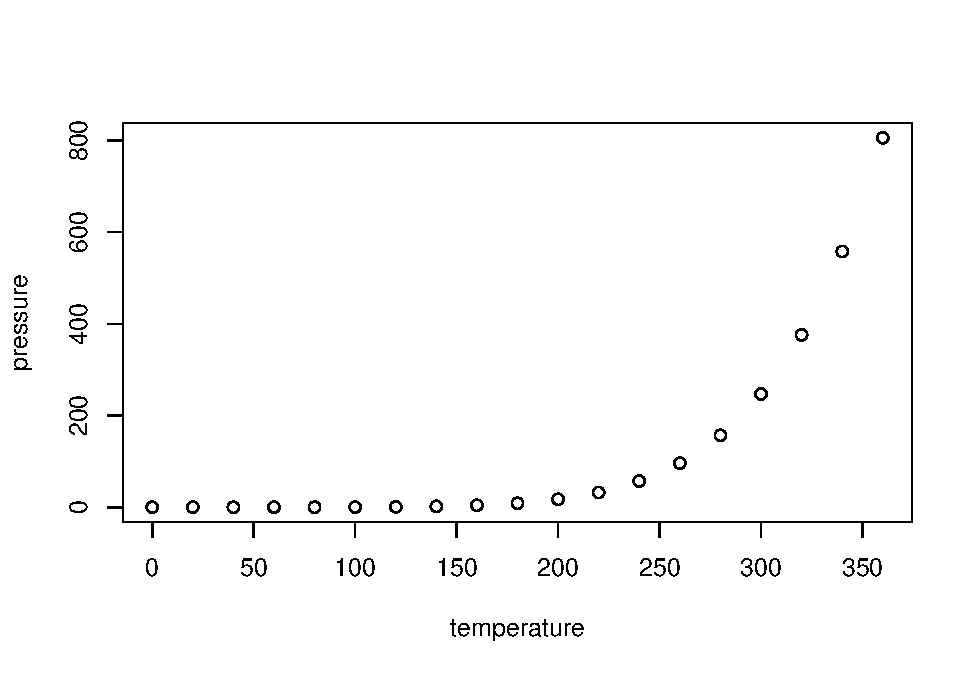
\includegraphics{week1_practice_files/figure-latex/pressure-1.pdf}

\begin{Shaded}
\begin{Highlighting}[]
\FunctionTok{library}\NormalTok{(tidyverse)}
\end{Highlighting}
\end{Shaded}

\begin{verbatim}
## Warning: package 'tidyverse' was built under R version 4.1.2
\end{verbatim}

\begin{verbatim}
## -- Attaching packages --------------------------------------- tidyverse 1.3.1 --
\end{verbatim}

\begin{verbatim}
## v ggplot2 3.3.5     v purrr   0.3.4
## v tibble  3.1.2     v dplyr   1.0.7
## v tidyr   1.1.3     v stringr 1.4.0
## v readr   1.4.0     v forcats 0.5.1
\end{verbatim}

\begin{verbatim}
## Warning: package 'ggplot2' was built under R version 4.1.2
\end{verbatim}

\begin{verbatim}
## -- Conflicts ------------------------------------------ tidyverse_conflicts() --
## x dplyr::filter() masks stats::filter()
## x dplyr::lag()    masks stats::lag()
\end{verbatim}

\begin{Shaded}
\begin{Highlighting}[]
\FunctionTok{library}\NormalTok{(openintro)}
\end{Highlighting}
\end{Shaded}

\begin{verbatim}
## Warning: package 'openintro' was built under R version 4.1.2
\end{verbatim}

\begin{verbatim}
## Loading required package: airports
\end{verbatim}

\begin{verbatim}
## Warning: package 'airports' was built under R version 4.1.2
\end{verbatim}

\begin{verbatim}
## Loading required package: cherryblossom
\end{verbatim}

\begin{verbatim}
## Warning: package 'cherryblossom' was built under R version 4.1.2
\end{verbatim}

\begin{verbatim}
## Loading required package: usdata
\end{verbatim}

\begin{verbatim}
## Warning: package 'usdata' was built under R version 4.1.2
\end{verbatim}

\begin{Shaded}
\begin{Highlighting}[]
\FunctionTok{data}\NormalTok{(}\StringTok{\textquotesingle{}arbuthnot\textquotesingle{}}\NormalTok{, }\AttributeTok{package=}\StringTok{\textquotesingle{}openintro\textquotesingle{}}\NormalTok{)}
\end{Highlighting}
\end{Shaded}

\begin{Shaded}
\begin{Highlighting}[]
\NormalTok{arbuthnot}
\end{Highlighting}
\end{Shaded}

\begin{verbatim}
## # A tibble: 82 x 3
##     year  boys girls
##    <int> <int> <int>
##  1  1629  5218  4683
##  2  1630  4858  4457
##  3  1631  4422  4102
##  4  1632  4994  4590
##  5  1633  5158  4839
##  6  1634  5035  4820
##  7  1635  5106  4928
##  8  1636  4917  4605
##  9  1637  4703  4457
## 10  1638  5359  4952
## # ... with 72 more rows
\end{verbatim}

\begin{Shaded}
\begin{Highlighting}[]
\FunctionTok{glimpse}\NormalTok{(arbuthnot)}
\end{Highlighting}
\end{Shaded}

\begin{verbatim}
## Rows: 82
## Columns: 3
## $ year  <int> 1629, 1630, 1631, 1632, 1633, 1634, 1635, 1636, 1637, 1638, 1639~
## $ boys  <int> 5218, 4858, 4422, 4994, 5158, 5035, 5106, 4917, 4703, 5359, 5366~
## $ girls <int> 4683, 4457, 4102, 4590, 4839, 4820, 4928, 4605, 4457, 4952, 4784~
\end{verbatim}

\hypertarget{some-exploration}{%
\section{Some Exploration:}\label{some-exploration}}

\hypertarget{to-access-the-data-in-a-single-column}{%
\subsection{To access the data in a single
column}\label{to-access-the-data-in-a-single-column}}

\begin{Shaded}
\begin{Highlighting}[]
\NormalTok{arbuthnot}\SpecialCharTok{$}\NormalTok{boys}
\end{Highlighting}
\end{Shaded}

\begin{verbatim}
##  [1] 5218 4858 4422 4994 5158 5035 5106 4917 4703 5359 5366 5518 5470 5460 4793
## [16] 4107 4047 3768 3796 3363 3079 2890 3231 3220 3196 3441 3655 3668 3396 3157
## [31] 3209 3724 4748 5216 5411 6041 5114 4678 5616 6073 6506 6278 6449 6443 6073
## [46] 6113 6058 6552 6423 6568 6247 6548 6822 6909 7577 7575 7484 7575 7737 7487
## [61] 7604 7909 7662 7602 7676 6985 7263 7632 8062 8426 7911 7578 8102 8031 7765
## [76] 6113 8366 7952 8379 8239 7840 7640
\end{verbatim}

\#Exercise 1: to extract just the counts of girls baptized?

\begin{Shaded}
\begin{Highlighting}[]
\FunctionTok{count}\NormalTok{(arbuthnot, }\StringTok{"girls"}\NormalTok{)}
\end{Highlighting}
\end{Shaded}

\begin{verbatim}
## # A tibble: 1 x 2
##   `"girls"`     n
##   <chr>     <int>
## 1 girls        82
\end{verbatim}

\hypertarget{below-is-the-vector-prsentation-of-count}{%
\subsection{Below is the vector prsentation of
count}\label{below-is-the-vector-prsentation-of-count}}

\begin{Shaded}
\begin{Highlighting}[]
\NormalTok{arbuthnot}\SpecialCharTok{$}\NormalTok{girls}
\end{Highlighting}
\end{Shaded}

\begin{verbatim}
##  [1] 4683 4457 4102 4590 4839 4820 4928 4605 4457 4952 4784 5332 5200 4910 4617
## [16] 3997 3919 3395 3536 3181 2746 2722 2840 2908 2959 3179 3349 3382 3289 3013
## [31] 2781 3247 4107 4803 4881 5681 4858 4319 5322 5560 5829 5719 6061 6120 5822
## [46] 5738 5717 5847 6203 6033 6041 6299 6533 6744 7158 7127 7246 7119 7214 7101
## [61] 7167 7302 7392 7316 7483 6647 6713 7229 7767 7626 7452 7061 7514 7656 7683
## [76] 5738 7779 7417 7687 7623 7380 7288
\end{verbatim}

\hypertarget{data-visualization}{%
\section{Data Visualization:}\label{data-visualization}}

\hypertarget{simple-scatter-plot-of-the-number-of-girls-baptized-per-year-using-ggplot}{%
\subsection{simple scatter plot of the number of girls baptized per year
using
ggplot}\label{simple-scatter-plot-of-the-number-of-girls-baptized-per-year-using-ggplot}}

\begin{Shaded}
\begin{Highlighting}[]
\FunctionTok{ggplot}\NormalTok{(}\AttributeTok{data =}\NormalTok{ arbuthnot, }\FunctionTok{aes}\NormalTok{(}\AttributeTok{x =}\NormalTok{ year, }\AttributeTok{y =}\NormalTok{ girls)) }\SpecialCharTok{+} 
  \FunctionTok{geom\_point}\NormalTok{()}
\end{Highlighting}
\end{Shaded}

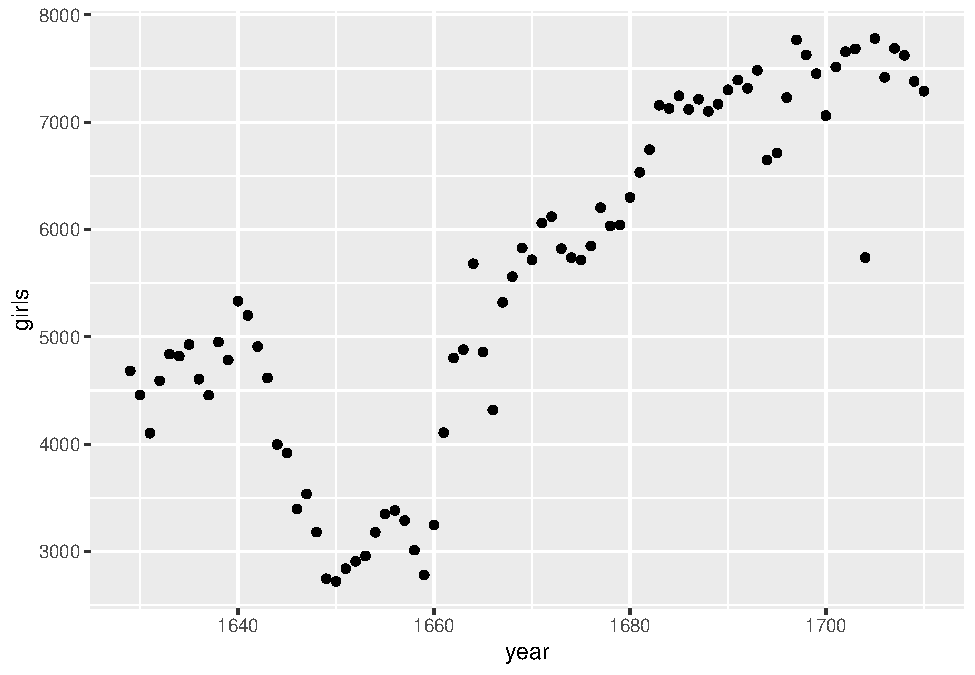
\includegraphics{week1_practice_files/figure-latex/unnamed-chunk-9-1.pdf}
\#\# simple line plot of the number of girls baptized per year using
ggplot

\begin{Shaded}
\begin{Highlighting}[]
\FunctionTok{ggplot}\NormalTok{(}\AttributeTok{data =}\NormalTok{ arbuthnot, }\FunctionTok{aes}\NormalTok{(}\AttributeTok{x =}\NormalTok{ year, }\AttributeTok{y =}\NormalTok{ girls)) }\SpecialCharTok{+} 
  \FunctionTok{geom\_line}\NormalTok{()}
\end{Highlighting}
\end{Shaded}

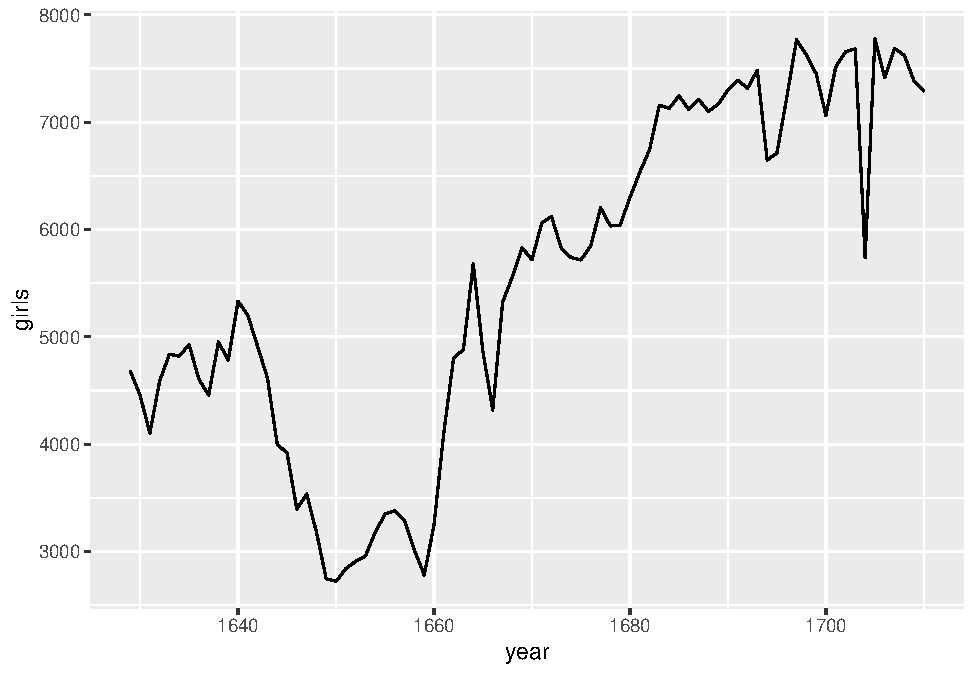
\includegraphics{week1_practice_files/figure-latex/unnamed-chunk-10-1.pdf}
\#\# Exercise 2: From 1640 to 1660 there is drop in the number of girls
baptized per year. \#\# From 1660 to 1700 there is a prominant increase
in the number of girls baptized per year.

\begin{Shaded}
\begin{Highlighting}[]
\NormalTok{arbuthnot}\SpecialCharTok{$}\NormalTok{boys }\SpecialCharTok{+}\NormalTok{ arbuthnot}\SpecialCharTok{$}\NormalTok{girls}
\end{Highlighting}
\end{Shaded}

\begin{verbatim}
##  [1]  9901  9315  8524  9584  9997  9855 10034  9522  9160 10311 10150 10850
## [13] 10670 10370  9410  8104  7966  7163  7332  6544  5825  5612  6071  6128
## [25]  6155  6620  7004  7050  6685  6170  5990  6971  8855 10019 10292 11722
## [37]  9972  8997 10938 11633 12335 11997 12510 12563 11895 11851 11775 12399
## [49] 12626 12601 12288 12847 13355 13653 14735 14702 14730 14694 14951 14588
## [61] 14771 15211 15054 14918 15159 13632 13976 14861 15829 16052 15363 14639
## [73] 15616 15687 15448 11851 16145 15369 16066 15862 15220 14928
\end{verbatim}

\hypertarget{adding-a-new-variable-to-the-dataframe}{%
\subsection{Adding a new variable to the
dataframe}\label{adding-a-new-variable-to-the-dataframe}}

\begin{Shaded}
\begin{Highlighting}[]
\NormalTok{arbuthnot }\OtherTok{\textless{}{-}}\NormalTok{ arbuthnot }\SpecialCharTok{\%\textgreater{}\%}
  \FunctionTok{mutate}\NormalTok{(}\AttributeTok{total =}\NormalTok{ boys }\SpecialCharTok{+}\NormalTok{ girls)}
\NormalTok{arbuthnot}
\end{Highlighting}
\end{Shaded}

\begin{verbatim}
## # A tibble: 82 x 4
##     year  boys girls total
##    <int> <int> <int> <int>
##  1  1629  5218  4683  9901
##  2  1630  4858  4457  9315
##  3  1631  4422  4102  8524
##  4  1632  4994  4590  9584
##  5  1633  5158  4839  9997
##  6  1634  5035  4820  9855
##  7  1635  5106  4928 10034
##  8  1636  4917  4605  9522
##  9  1637  4703  4457  9160
## 10  1638  5359  4952 10311
## # ... with 72 more rows
\end{verbatim}

\hypertarget{exercise-3-to-generate-a-plot-of-the-proportion-of-boys-born-over-time}{%
\subsection{Exercise 3: To generate a plot of the proportion of boys
born over
time}\label{exercise-3-to-generate-a-plot-of-the-proportion-of-boys-born-over-time}}

\begin{Shaded}
\begin{Highlighting}[]
\NormalTok{arbuthnot }\OtherTok{\textless{}{-}}\NormalTok{ arbuthnot }\SpecialCharTok{\%\textgreater{}\%}
  \FunctionTok{mutate}\NormalTok{(}\AttributeTok{boy\_ratio =}\NormalTok{ boys}\SpecialCharTok{/}\NormalTok{total)}
\NormalTok{arbuthnot}
\end{Highlighting}
\end{Shaded}

\begin{verbatim}
## # A tibble: 82 x 5
##     year  boys girls total boy_ratio
##    <int> <int> <int> <int>     <dbl>
##  1  1629  5218  4683  9901     0.527
##  2  1630  4858  4457  9315     0.522
##  3  1631  4422  4102  8524     0.519
##  4  1632  4994  4590  9584     0.521
##  5  1633  5158  4839  9997     0.516
##  6  1634  5035  4820  9855     0.511
##  7  1635  5106  4928 10034     0.509
##  8  1636  4917  4605  9522     0.516
##  9  1637  4703  4457  9160     0.513
## 10  1638  5359  4952 10311     0.520
## # ... with 72 more rows
\end{verbatim}

\hypertarget{analysis-you-can-see-that-there-is-a-consistant-balance-in-the-rise-and-fall-pattern-of-boys-ratio-per-year}{%
\subsection{Analysis: You can see that there is a consistant balance in
the rise and fall pattern of boys ratio per
year}\label{analysis-you-can-see-that-there-is-a-consistant-balance-in-the-rise-and-fall-pattern-of-boys-ratio-per-year}}

\begin{Shaded}
\begin{Highlighting}[]
\FunctionTok{ggplot}\NormalTok{(}\AttributeTok{data =}\NormalTok{ arbuthnot, }\FunctionTok{aes}\NormalTok{(}\AttributeTok{x =}\NormalTok{ year, }\AttributeTok{y =}\NormalTok{ boy\_ratio)) }\SpecialCharTok{+} 
  \FunctionTok{geom\_line}\NormalTok{()}
\end{Highlighting}
\end{Shaded}

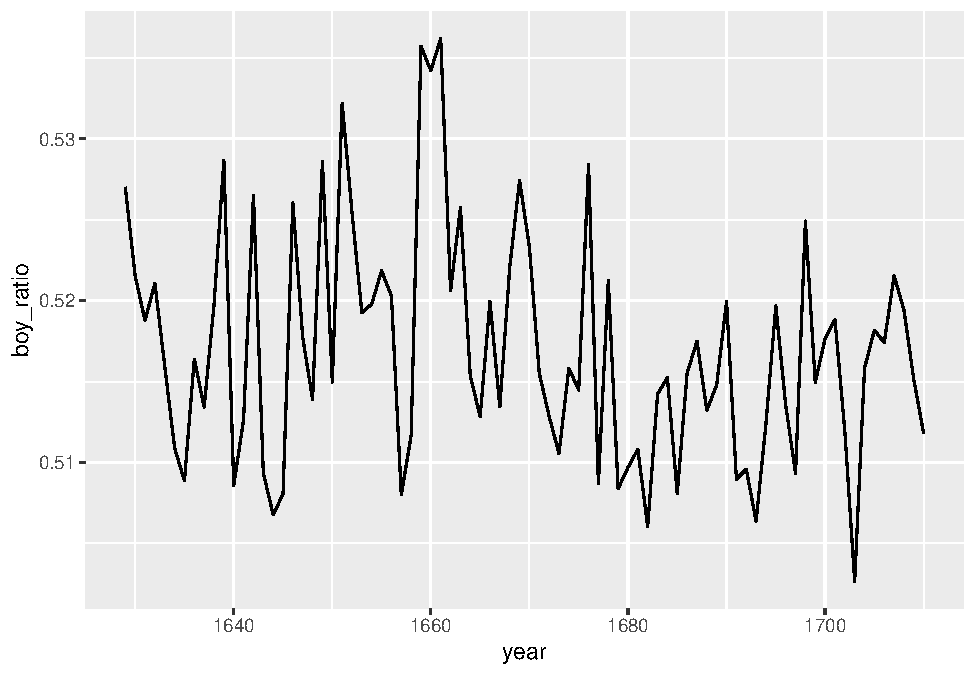
\includegraphics{week1_practice_files/figure-latex/unnamed-chunk-14-1.pdf}

\begin{Shaded}
\begin{Highlighting}[]
\FunctionTok{ggplot}\NormalTok{(}\AttributeTok{data =}\NormalTok{ arbuthnot, }\FunctionTok{aes}\NormalTok{(}\AttributeTok{x =}\NormalTok{ year, }\AttributeTok{y =}\NormalTok{ girls)) }\SpecialCharTok{+} 
  \FunctionTok{geom\_point}\NormalTok{()}
\end{Highlighting}
\end{Shaded}

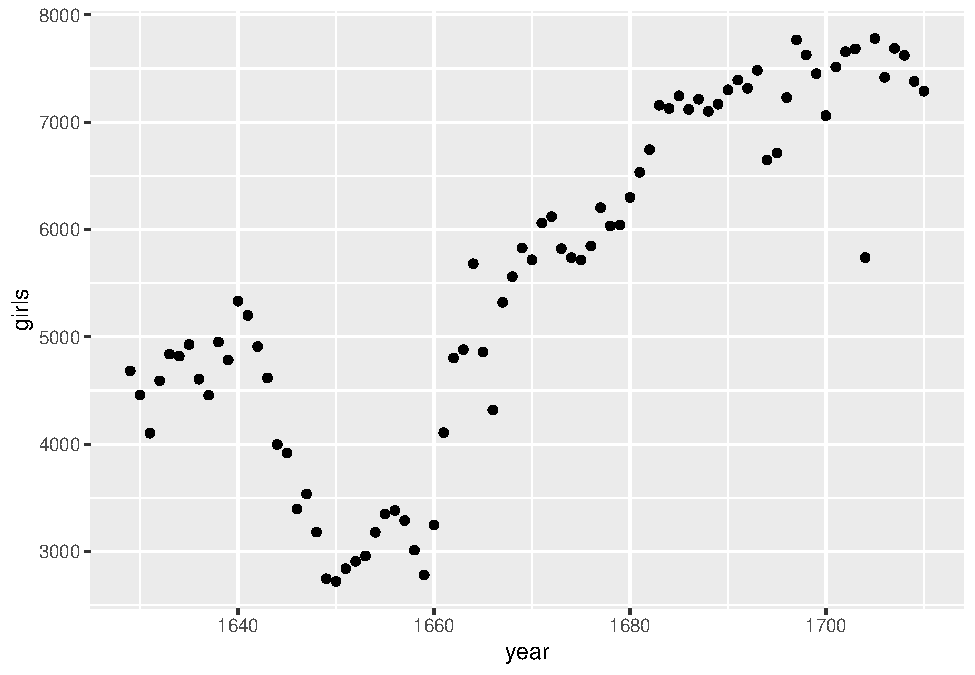
\includegraphics{week1_practice_files/figure-latex/unnamed-chunk-15-1.pdf}

\begin{Shaded}
\begin{Highlighting}[]
\NormalTok{arbuthnot }\OtherTok{\textless{}{-}}\NormalTok{ arbuthnot }\SpecialCharTok{\%\textgreater{}\%}
  \FunctionTok{mutate}\NormalTok{(}\AttributeTok{boy\_to\_girl\_ratio =}\NormalTok{ boys }\SpecialCharTok{/}\NormalTok{ girls)}
\NormalTok{arbuthnot}
\end{Highlighting}
\end{Shaded}

\begin{verbatim}
## # A tibble: 82 x 6
##     year  boys girls total boy_ratio boy_to_girl_ratio
##    <int> <int> <int> <int>     <dbl>             <dbl>
##  1  1629  5218  4683  9901     0.527              1.11
##  2  1630  4858  4457  9315     0.522              1.09
##  3  1631  4422  4102  8524     0.519              1.08
##  4  1632  4994  4590  9584     0.521              1.09
##  5  1633  5158  4839  9997     0.516              1.07
##  6  1634  5035  4820  9855     0.511              1.04
##  7  1635  5106  4928 10034     0.509              1.04
##  8  1636  4917  4605  9522     0.516              1.07
##  9  1637  4703  4457  9160     0.513              1.06
## 10  1638  5359  4952 10311     0.520              1.08
## # ... with 72 more rows
\end{verbatim}

\hypertarget{to-see-the-boolean-output-if-the-boys-are-more-than-girls}{%
\subsection{To see the boolean output if the boys are more than
girls}\label{to-see-the-boolean-output-if-the-boys-are-more-than-girls}}

\begin{Shaded}
\begin{Highlighting}[]
\NormalTok{arbuthnot }\OtherTok{\textless{}{-}}\NormalTok{ arbuthnot }\SpecialCharTok{\%\textgreater{}\%}
  \FunctionTok{mutate}\NormalTok{(}\AttributeTok{more\_boys =}\NormalTok{ boys }\SpecialCharTok{\textgreater{}}\NormalTok{ girls)}
\NormalTok{arbuthnot}
\end{Highlighting}
\end{Shaded}

\begin{verbatim}
## # A tibble: 82 x 7
##     year  boys girls total boy_ratio boy_to_girl_ratio more_boys
##    <int> <int> <int> <int>     <dbl>             <dbl> <lgl>    
##  1  1629  5218  4683  9901     0.527              1.11 TRUE     
##  2  1630  4858  4457  9315     0.522              1.09 TRUE     
##  3  1631  4422  4102  8524     0.519              1.08 TRUE     
##  4  1632  4994  4590  9584     0.521              1.09 TRUE     
##  5  1633  5158  4839  9997     0.516              1.07 TRUE     
##  6  1634  5035  4820  9855     0.511              1.04 TRUE     
##  7  1635  5106  4928 10034     0.509              1.04 TRUE     
##  8  1636  4917  4605  9522     0.516              1.07 TRUE     
##  9  1637  4703  4457  9160     0.513              1.06 TRUE     
## 10  1638  5359  4952 10311     0.520              1.08 TRUE     
## # ... with 72 more rows
\end{verbatim}

\begin{Shaded}
\begin{Highlighting}[]
\NormalTok{arbuthnot }\SpecialCharTok{\%\textgreater{}\%}
  \FunctionTok{summarize}\NormalTok{(}\AttributeTok{min =} \FunctionTok{min}\NormalTok{(boys), }\AttributeTok{max =} \FunctionTok{max}\NormalTok{(boys))}
\end{Highlighting}
\end{Shaded}

\begin{verbatim}
## # A tibble: 1 x 2
##     min   max
##   <int> <int>
## 1  2890  8426
\end{verbatim}

\hypertarget{assignment-2}{%
\section{Assignment 2:}\label{assignment-2}}

\hypertarget{for-present-day-birth-records-in-the-united-states}{%
\subsection{For present day birth records in the United
States}\label{for-present-day-birth-records-in-the-united-states}}

\begin{Shaded}
\begin{Highlighting}[]
\FunctionTok{data}\NormalTok{(}\StringTok{\textquotesingle{}present\textquotesingle{}}\NormalTok{, }\AttributeTok{package=}\StringTok{\textquotesingle{}openintro\textquotesingle{}}\NormalTok{)}
\NormalTok{present}
\end{Highlighting}
\end{Shaded}

\begin{verbatim}
## # A tibble: 63 x 3
##     year    boys   girls
##    <dbl>   <dbl>   <dbl>
##  1  1940 1211684 1148715
##  2  1941 1289734 1223693
##  3  1942 1444365 1364631
##  4  1943 1508959 1427901
##  5  1944 1435301 1359499
##  6  1945 1404587 1330869
##  7  1946 1691220 1597452
##  8  1947 1899876 1800064
##  9  1948 1813852 1721216
## 10  1949 1826352 1733177
## # ... with 53 more rows
\end{verbatim}

Note that the \texttt{echo\ =\ FALSE} parameter was added to the code
chunk to prevent printing of the R code that generated the plot.

\end{document}
